\documentclass[12pt]{scrartcl}
\usepackage[sexy]{evan}
\usepackage{graphicx,amsmath,amssymb,amsthm,amsfonts,babel}
\usepackage{tikz, tkz-euclide}
\usepackage{lipsum}
\usepackage{setspace}
\graphicspath{ {./} }
\usetikzlibrary{calc,through,intersections}
\usepackage[paperwidth=16cm, paperheight=16cm,margin=1cm]{geometry}

\colorlet{EvanRed}{Red!50!Purple}

\newcommand{\siku}[4][.5cm]
	{
	\coordinate (tempa) at ($(#3)!#1!(#2)$);
	\coordinate (tempb) at ($(#3)!#1!(#4)$);
	\coordinate (tempc) at ($(tempa)!0.5!(tempb)$);%midpoint
	\draw[black] (tempa) -- ($(#3)!2!(tempc)$) -- (tempb);
	}
	\usetikzlibrary{calc,positioning,intersections}

\setstretch{1.5}

\usepackage{etoolbox}
\newcommand{\zerodisplayskips}{%
  \setlength{\abovedisplayskip}{5pt}%
  \setlength{\belowdisplayskip}{5pt}%
  \setlength{\abovedisplayshortskip}{5pt}%
  \setlength{\belowdisplayshortskip}{5pt}}
\appto{\normalsize}{\zerodisplayskips}
\appto{\small}{\zerodisplayskips}
\appto{\footnotesize}{\zerodisplayskips}
\setlength\parindent{10pt}

\title{Pembahasan OSN-K 2023 part 1/n}
\author{by Azzam L.H}
\date{}


\begin{document}
\maketitle
\pagestyle{plain}
\vspace{-1.5cm}


\section{Nomor 1 Kemampuan Dasar}
Hasil penjumlahan semua solusi persamaan
\begin{align*}
|x-|2x+6||=99
\end{align*}
adalah \dots
\begin{solusi}
Bagi kasus untuk $x \ge -\tfrac{6}{2}$ atau $x < -\tfrac{6}{2}$.

Jika $x \ge -\tfrac{6}{2}$, maka $|2x+6| = 2x+6$. Jelas bahwa $x > -6$ sehingga $|x+6|=x+6$ yang mana
$$99=|x-|2x+6||=|x-(2x+6)|=|-x-6|=|x+6|=x+6 \implies x = 93.$$

Jika $x < -\tfrac{6}{2}$, maka $|2x+6| = -2x-6$. Maka
$$99=|x-|2x+6||=|x-(-2x-6)|=|3x+6|=3|x+6| \implies 33=|x+2|.$$
Akan dibagi kasus lagi:
\begin{itemize}
\item Jika $x \ge -2$ sehingga $|x+2|=x+2$ maka $33=x+2 \implies x=31$. Solusi ini tidak memenuhi karena harusnya $-2 \le x < -\tfrac{6}{2}$.
\item Jika $x \ge -2$ sehingga $|x+2|=-(x+2)$ maka $33=-x-2 \implies x=-35$.
\end{itemize}
Cek semua solusi diatas, hanya $x=93$ dan $x=-35$ yang memenuhi. Berarti hasil penjumlahan semua solusinya adalah $93+(-35)=\boxed{58}$.

\end{solusi}

\section{Nomor 1 Kemampuan Lanjut}
Diberikan segiempat $ABCD$ siklis dengan lingkaran luarnya adalah $\omega$. Panjang $BC=CD$, $AC$ memotong $BD$ di titik $E$, $BE=7$, dan $DE=4$. Garis singgung $\omega$ di titik $A$ memotong $BD$ di titik $P$. Jika $\frac{PD}{PB}$ dapat ditulis dalam bentuk $\frac{m}{n}$ dengan $m$ dan $n$ adalah bilangan asli yang saling relatif prima, tentukan nilai dari $m+n$.
\begin{solusi}
Perhatikan bahwa panjang busur $BC=CD$ sehingga $\angle CAB = \angle DAC$. Oleh karena itu, $AE$ adalah garis bagi dalam $\angle BAD$ segitiga $BAD$ sehingga dengan Teorema Garis bagi kita punya $\frac{AD}{BA}=\frac{4}{7}$.
\begin{center}
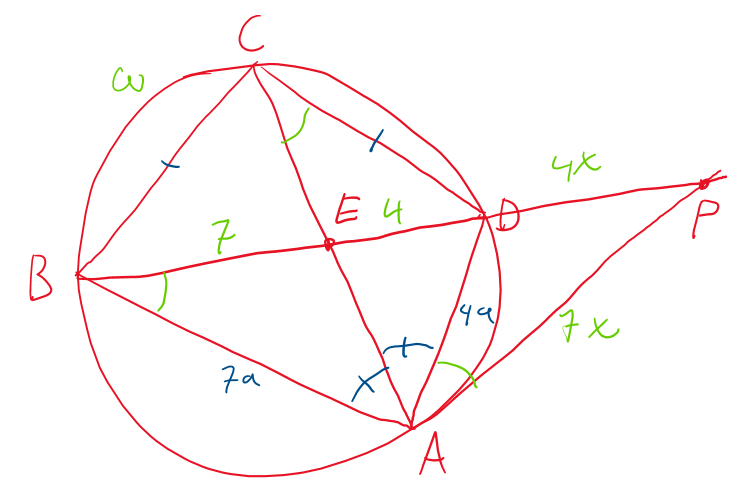
\includegraphics[scale=0.5]{1KL}
\end{center}
Sekarang, dari Alternate Segment Theorem, $\angle PAD = \angle ABP$. Karena diketahui juga $\angle DPA = \angle BPA$ maka didapatkan $\triangle DPA \sim \triangle \triangle APB$. Oleh karena itu, kita punya
$$\frac{PA}{PD} = \frac{AD}{BA} = \frac{4}{7}.$$
Berarti dapat dimisalkan $DP=4x$ dan $PA=7x$. Dari sini dengan Power of a Point, kita punya
$$PD \cdot PB = PA^2 \implies (4x)(4x+11) = (7x)^2 \implies x = \frac{4}{3}.$$
Dari fakta tersebut, $\frac{PD}{PB} = \frac{4x}{4x+11}=\frac{16}{49}$ yang menyebabkan $m=16$ dan $n=49$ sehingga $m+n=\boxed{65}$.
\end{solusi}

\section{Nomor 9 Kemampuan Lanjut}
Diberikan segitiga $ABC$. Misal titik $D,E,F$ terletak pada sisi $BC,CA,AB$ sehingga $AD,BE,CF$ berpotongan di satu titik. Diketahui bahwa $\angle EDF = 56^\circ$. Jika $\angle ADB = 90^\circ$ dan $AF=FB$, maka besar sudut $\angle ABC$ adalah \dots
\begin{solusi}.
\begin{center}
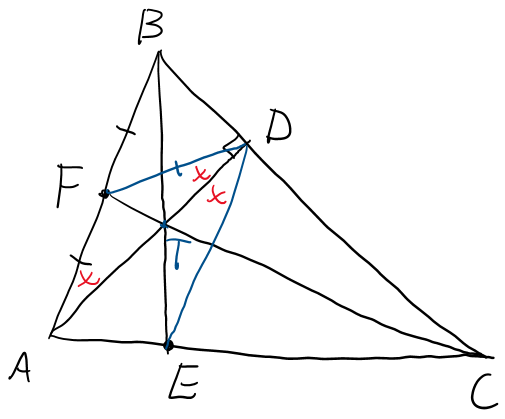
\includegraphics[scale=0.5]{9KL}
\end{center}

 Perhatikan karena $AF=FB$ dan $\angle ADB = 90^\circ$, maka $DF=FA$. Berarti jika dimisalkan $\angle FDA = x$ maka $\angle FAD = \angle FDA = x$. 

Sekarang perhatikan karena $AD,BE,CF$ bertemu di satu titik dan $\frac{BF}{FA}=1$ maka dengan Teorema Ceva
$$\frac{BF}{FA}\cdot \frac{AE}{EC} \cdot \frac{CD}{DB} = 1 \implies \frac{AE}{EC} = \frac{DB}{CD} \implies DE \parallel BA.$$
Dari sini, karena $DE \parallel BA$ maka $\angle EDA = \angle DAF = x$. Hal tersebut mengakibatkan $56^\circ =\angle EDF = 2x \implies x = 28^\circ$. Berarti kita akan mendapat $\angle ABC = 90^\circ - \angle BAD = 90^\circ - x = \boxed{62^\circ}.$
\end{solusi}


\end{document}
